% ------------------------------------------------------------------------
% ------------------------------------------------------------------------
% Relatório de Trabalho 3 de Estrutura de Dados II
% Autores: André Barreto e Igor Ventorim
% ------------------------------------------------------------------------
% ------------------------------------------------------------------------

\documentclass[
	11pt,				% tamanho da fonte
	oneside,			% para impressão apenas no verso. Oposto a twoside
	a4paper,			% tamanho do papel. 
	english,			% idioma adicional para hifenização
	brazil,				% o último idioma é o principal do documento
	]{article}


% ---
% PACOTES
% ---
\usepackage{lmodern}			% Usa a fonte Latin Modern
\usepackage[T1]{fontenc}		% Selecao de codigos de fonte.
\usepackage[utf8]{inputenc}		% Codificacao do documento (conversão automática dos acentos)
\usepackage{indentfirst}		% Indenta o primeiro parágrafo de cada seção.
\usepackage{nomencl} 			% Lista de simbolos
\usepackage{color}				% Controle das cores
\usepackage{graphicx}			% Inclusão de gráficos
\usepackage{microtype} 			% para melhorias de justificação
\usepackage{makeidx}			% Gerar índice
\usepackage{multirow,tabularx}
\usepackage{multicol}
\usepackage{listings}			% Include the listings-package
\usepackage{color}
\usepackage{hyperref}
\usepackage{cite}
\usepackage{url}
\usepackage[brazilian]{babel}
\usepackage[brazilian,hyperpageref]{backref}	 % Paginas com as citações na bibl
\usepackage{amsmath}
\usepackage{pgfplots}

\usepackage{lipsum}
% ---

% ---
% Configurações do pacote listings
% ---
\definecolor{mygreen}{rgb}{0,0.6,0}
\definecolor{mygray}{rgb}{0.571428571,0.571428571,0.571428571}
\definecolor{mymauve}{rgb}{0.5714285718,0,0.82}
\definecolor{codegreen}{rgb}{0,0.6,0}
\definecolor{codegray}{rgb}{0.571428571,0.571428571,0.571428571}
\definecolor{codepurple}{rgb}{0.5714285718,0,0.82}
\definecolor{backcolour}{rgb}{0.95,0.95,0.92}
\lstset{
	backgroundcolor=\color{white},   % choose the background color; you must add \usepackage{color} or \usepackage{xcolor}
	basicstyle=\footnotesize,        % the size of the fonts that are used for the code
	breakatwhitespace=false,         % sets if automatic breaks should only happen at whitespace
	breaklines=true,                 % sets automatic line breaking
	captionpos=b,                    % sets the caption-position to bottom
	commentstyle=\color{mygreen},    % comment style
	deletekeywords={...},            % if you want to delete keywords from the given language
	escapeinside={\%*}{*)},          % if you want to add LaTeX within your code
	extendedchars=true,              % lets you use non-ASCII characters; for 8-bits encodings only, does not work with UTF-8
	keepspaces=true,                 % keeps spaces in text, useful for keeping indentation of code (possibly needs columns=flexible)
	keywordstyle=\color{blue},       % keyword style
	language=C,                      % the language of the code
	otherkeywords={*,...},           % if you want to add more keywords to the set
	numbers=left,                    % where to put the line-numbers; possible values are (none, left, right)
	numbersep=5pt,                   % how far the line-numbers are from the code
	numberstyle=\tiny\color{mygray}, % the style that is used for the line-numbers
	rulecolor=\color{black},         % if not set, the frame-color may be changed on line-breaks within not-black text (e.g. comments (green here))
	showspaces=false,                % show spaces everywhere adding particular underscores; it overrides 'showstringspaces'
	showstringspaces=false,          % underline spaces within strings only
	showtabs=false,                  % show tabs within strings adding particular underscores
	stepnumber=1,                    % the step between two line-numbers. If it's 1, each line will be numbered
	stringstyle=\color{mymauve},     % string literal style
	tabsize=2,	                   % sets default tabsize to 2 spaces
	title=\lstname                   % show the filename of files included with \lstinputlisting; also try caption instead of title
}
% ---
	
% ---
% Informações de dados para CAPA
% ---
\title{\textbf{Solução de Problemas de Valor no Contorno Bidimensionais}}
\author{
André Barreto e Igor Ventorim\\\\
\normalsize Universidade Federal do Espírito Santo\\
}
\date{2015}
% ---

% ---
% Configurações de aparência do PDF final
% ---
\definecolor{blue}{RGB}{41,5,195}

% informações do PDF
\makeatletter
\hypersetup{
	pdftitle={\@title}, 
	pdfauthor={\@author},
	pdfsubject={Escalonamento de Jobs},
	pdfcreator={LaTeX with abnTeX2},
	pdfkeywords={abnt}{latex}{abntex}{abntex2}{atigo científico}, 
	colorlinks=true,       		% false: boxed links; true: colored links
	linkcolor=blue,          	% color of internal links
	citecolor=blue,        		% color of links to bibliography
	filecolor=magenta,      	% color of file links
	urlcolor=blue,
	bookmarksdepth=4
}
\makeatother
% --- 

% ---
% Compila o indice
% ---
\makeindex
% ---

% --- 
% Espaçamentos entre linhas e parágrafos 
% --- 
\setlength{\parindent}{1.3cm}
\setlength{\parskip}{0.2cm}  % tente também \onelineskip
% ---

% ----
% Início do documento
% ----
\begin{document}

% Seleciona o idioma do documento
\selectlanguage{brazil}

% Retira espaço extra obsoleto entre as frases.
\frenchspacing

\graphicspath{ {Imagens/} }

% ----------------------------------------------------------
% Página de Título
% ----------------------------------------------------------
\begin{titlepage}
	\centering
	{\scshape \large Universidade Federal do Espírito Santo\par}
	{\large Departamento de Informática\par}
	\vspace{1cm}
	{\large André Barreto\par}
	{\large Igor Ventorim\par}
	
	\vfill
	{\LARGE \bfseries Solução de Problemas de Valor no Contorno Bidimensionais\par}
	\vspace{1cm}
	{\large Trabalho 2 de Algoritmos Numéricos\par}

	\vfill

	{\large Vitória\par}
	{\large 2015\par}
\end{titlepage}
\addtocounter{page}{1}

% ----------------------------------------------------------
% Introdução
% ----------------------------------------------------------
\section{Introdução}
Equações diferenciais parciais, aparecem com frequência na solução de problemas em diversas a áreas do conhecimento. Sendo assim, vamos estudar o processo de discretização pelo método das diferenças finitas de equações do tipo:

\begin{equation} \label{eq:1}
- \left(\frac{\partial^2 u}{\partial x^2} + \frac{\partial^2 u}{\partial y^2}\right) +
a\frac{\partial u}{\partial x} +
b\frac{\partial u}{\partial y} +
cu = f(x,y) \text{ em } \Omega
\end{equation}

\noindent considerando que \textit{a, b, c e f(x,y)} são conhecidas e que $u(x,y)$ é conhecida no contorno de $\Omega$. Deseja-se obter a solução $u(x,y)$ no interior de um domínio retangular de dimensões $(x_0,x_{N+1}) \times (y_0,y_{M+1})$, sendo conhecida a solução no contorno do retângulo (condições de Dirichlet). Considere uma subdivisão do domínio em células retangulares, sendo $N+1$ divisões na horizontal e $M+1$ divisões na vertical, respectivamente, de dimensões $h_x$ e $h_y$.

Este trabalho tem como objetivo discretizar a equação \eqref{eq:1} pelo método das diferenças finitas e resolver o sistema linear resultante através dos métodos de Eliminação Gaussiana e Gauss-Seidel com relaxação sucessiva (SOR). Os algoritmos devem ser implementados tanto em linguagem C como em Octave.

Será feita uma análise comparativa dos métodos de solução considerados e das linguagens utilizadas.

Além disso, serão utilizadas técnicas de armazenamento e resolução de matrizes esparsas, ou seja, salvando apenas os elementos indispensáveis para a resolução de do sistema linear.

% ----------------------------------------------------------
% Referencial Teórico
% ----------------------------------------------------------
\section{Referencial Teórico}
A discretização da equação \eqref{eq:1} resulta em um sistema linear cuja matriz de coeficientes é uma matriz penta-diagonal \cite{bvp}, como ilustrado a seguir.

$
\begin{pmatrix}
	a_1     & c_1     &         & e_1     &         &         &         &         &         \\
	b_2     & a_2     & c_2     &         & e_2     &         &         &         &         \\
	        & \ddots  & \ddots  & \ddots  &         & \ddots  &         &         &         \\
	d_{n+1} &         & b_{n+1} & a_{n+1} & c_{n+1} &         & e_{n+1} &         &         \\
	        & \ddots  &         & \ddots  & \ddots  & \ddots  &         & \ddots  &         \\
	        &         & d_I     &         & b_I     & a_I     & c_I     &         & e_I     \\
	        &         &         & \ddots  &         & \ddots  & \ddots  & \ddots  &         \\
	        &         &         & d_{N-1} &         &         & b_{N-1} & a_{N-1} & c_{N-1} \\
	        &         &         &         & d_N     &         &         & b_N     & a_N     \\
\end{pmatrix}
$

Para a resolução do sistema linear penta-diagonal resultante após o processamento dos dados de entrada, serão utilizadas os métodos de resolução adaptados à matrizes esparsas já implementados pelo trabalho anterior: Método de Gauss e SOR.

Neste trabalho, foram utilizadas diversas técnicas para a resolução. Em primeiro momento foram criadas funções requisitadas pelo trabalho e uma função de discretização ao qual considera N a quantidade de pontos X na malha e M a quantidade de pontos Y. Após isso serão armazenados $N \times M$ pontos. Uma função de criação da matriz, onde criamos a matriz penta diagonal, onde a,b,c são constantes. De tal forma que a matriz tenha todos os valores de A,B,C,D,E iguais.

Também é criado uma função de construção do vetor independente, ao qual foi utilizado a biblioteca \textit{ae} da linguagem lua e a função \textit{eval} de Octave, para que possa ser interpretada a função passada como parâmetro. Após isso são aplicados os pontos na função, montando o vetor independente. Tendo a matriz e o vetor independente foi substituído da matriz os pontos de contorno fornecidos, construindo assim o sistema esparso, onde, resolvendo ele, conseguimos adquirir os valores de $U(x,y)$.

Para resolver o sistema, foram utilizados o programa adquirido no trabalho passado e o \textit{sor} e \textit{gauss} do Octave vistos em sala. Desta forma foi possível encontrar o resultado de nossa equação em cada ponto discretizado.

% ----------------------------------------------------------
% Implementação
% ----------------------------------------------------------
\section{Implementação}
Este trabalho foi desenvolvido tanto em linguagem C quanto em Octave. Além disso, criamos uma interface gráfica em \textit{web} para facilitar a entrada de dados do usuário. Veja nesta seção as partes relevantes dos códigos e a apresentação da interface.

\subsection{Linguagem C}
Em linguagem C, criamos o seguinte programa principal que chama as principais funções para a resolução do problema:

\begin{lstlisting}[language=C, caption=Função \textit{main}]
int main(int argc, char **argv)
{
	(...)
	input = readData(&a, &b, &c);
	lPoints = createLPoints(input->amountX, input->amountY);
	discretiza(lPoints,input,&hx, &hy);
	matrix = createMatrix(input,a, b, c);
	vetorIndependent = createVIndependent(lPoints,input);
	insertContourn(matrix, vetorIndependent, input);
	writeMatrix(matrix, vetorIndependent,input);
	(...)
}
\end{lstlisting}

Após a chamadas destas funções, tem-se como resultado um matriz escrita em um arquivo em formato próprio para manipulação esparsa, que então é lido pelos algoritmos Gauss e SOR.

\subsubsection{Estruturas}
Para auxiliar na manipulação dos dados de entrada, foram criadas estas duas estruturas de armazenamento, explicitadas no código abaixo.

\begin{lstlisting}[language=C, caption=Estruturas de entrada]
typedef struct data
{
	double beginX;
	double endX;
	double beginY;
	double endY;
	int amountX;
	int amountY;
	int contour;
	Contour *elements;
} Data;

typedef struct contour
{
	int x;
	int y;
	double value;
} Contour;
\end{lstlisting}

Além destas, existe a estrutura \textit{Ponto}, que simplesmente armazena as coordenadas \textit{(x,y)}.

\subsubsection{Principais funções}

A função \textit{discretiza} é responsável por gerar o vetor de pontos discretizados a partir dos intervalos e números de subintervalos recebidos.
\begin{lstlisting}[language=C, caption=Função Discretiza]
void discretiza(Points *lPoints, Data *input)
{
	int i,j,pos = 0;
	double hx,hy;

	hx = (input->endX - input->beginX)/(double)input->amountX-1;
	hy = (input->endY - input->beginY)/(double)input->amountY-1;

	for( i = 1; i <= input->amountX;i++)
		for( j = 1; j <= input->amountY;j++)
		{
			lPoints[pos].x = input->beginX + (double)(j - 1)*(hx);
			lPoints[pos].y = input->beginY + (double)(i - 1)*(hy);
			pos++;
		}
}
\end{lstlisting}

A função \textit{createMatrix} gera uma matriz de tamanho $n \times n$ onde $n$ é a quantidade de elementos definidos pelos valores de entrada.
\begin{lstlisting}[language=C, caption=Função Cria Matriz]
double **createMatrix(Data *input,double a, double b, double c)
{
	double hx,hy, **matrix;
	double aI,bI,cI,dI,eI;
	int qtdElementos, i, j;

	qtdElementos = (input->amountX * input->amountY);

	hx = (input->endX - input->beginX)/(double)input->amountX-1;
	hy = (input->endY - input->beginY)/(double)input->amountY-1;

	aI = c + 2 *((1/(hx*hx)) + (1/(hy*hy)));
	bI = (-1/(hx*hx)) - (a/(2*hx));
	cI = (-1/(hx*hx)) + (a/(2*hx));
	dI = (-1/(hy*hy)) - (b/(2*hy));
	eI = (-1/(hy*hy)) + (b/(2*hy));

	matrix = calloc((size_t)qtdElementos,sizeof(double*));
	for(i = 0; i < qtdElementos; i++)
		matrix[i] = calloc((size_t)qtdElementos,sizeof(double));

	for(i = 0; i < qtdElementos; i++)
		for( j = 0; j < qtdElementos; j++)
		{
			if( i == j)
				matrix[i][j] = aI;
			else if ((j+1) == i)
				matrix[i][j] = bI;
			else if((j-1) == i)
				matrix[i][j] = cI;
			else if((j+input->amountX) == i)
				matrix[i][j] = dI;
			else if ((j-input->amountX) == i)
				matrix[i][j] = eI;
			else
				matrix[i][j] = 0;
		}

	return matrix;
}
\end{lstlisting}

A função \textit{insertContourn} atualiza a matriz penta-diagonal com os valores conhecidos do contorno.
\begin{lstlisting}[language=C, caption=Função Insere Contorno]
void insertContourn(double **matrix, double *vetIndependent, Data *input)
{
	int i,j, qtdElementos;
	int index;
	qtdElementos = (input->amountX * input->amountY);

	for( j = 0; j < input->contour;j++)
	{
		index = generatorNewIndex(input->elements[j].x,input->elements[j].y,input->amountX);
		vetIndependent[index] = input->elements[j].value;
		for(i = 0; i < qtdElementos ; i++)
		{
			if(i == index)
			{
				matrix[index][i] = 1;
			}else
				matrix[index][i] = 0;
		}
	}
}
\end{lstlisting}

Aplicadas as funções anteriores, é chamada a \textit{writeMatrix}, que escreve, em formato esparso, a matriz em um arquivo de saída.

\subsection{Octave}
Foi traduzido o procedimento da linguagem C apresentado para Octave.

\subsubsection{Principais funções}

\begin{lstlisting}[language=Octave, caption=Função Discretiza]
hx = (endX - matrixSparseeginX)/(tamX-1);
hy = (endY - matrixSparseeginY)/(tamY-1);
qtdElementos = tamX*tamY;
lPoints = zeros(qtdElementos,2);
pos = 1;
for i=1:tamX
  for j=1:tamY
    lPoints(pos,1) = matrixSparseeginX + (j-1)*hx;
    lPoints(pos,2) = matrixSparseeginY + (i-1)*hy;
    pos++;
  end
 end
\end{lstlisting}

\begin{lstlisting}[language=Octave, caption=Função Cria Matriz]
 matrix = zeros(qtdElementos,qtdElementos);
 aI = c + 2 *((1/(hx*hx)) + (1/(hy*hy)));
 matrixSparseI = (-1/(hx*hx)) - (a/(2*hx));
 cI = (-1/(hx*hx)) + (a/(2*hx));
 dI = (-1/(hy*hy)) - (matrixSparse/(2*hy));
 eI = (-1/(hy*hy)) + (matrixSparse/(2*hy));

 for i=1:qtdElementos
   for j=1:qtdElementos
     if i == j
       matrix(i,j) = aI;
     elseif (j+1) == i
       matrix(i,j) = matrixSparseI;
     elseif (j-1) == i
       matrix(i,j) = cI;
     elseif (j+tamX) == i
       matrix(i,j) = dI;
     elseif (j-tamY) == i
       matrix(i,j) = eI;
     else
       matrix(i,j) = 0;
      endif
   end
 end
\end{lstlisting}

\begin{lstlisting}[language=Octave, caption=Função Insere Contorno]
for j=1:contour
  index = A(j,1) + tamX * (A(j,2)-1);
  vetIndependent(index) = A(j,3);
  for i=1:qtdElementos
    if i == index
      matrix(index,i) = 1;
    else
      matrix(index,i) = 0;
    endif
  end
end
\end{lstlisting}

Após isto, também é chamada uma função para escrever a matriz em um arquivo de saída.

\subsection{Interface web}
A interface \textit{web} está localizada no endereço \url{http://antrab2.inf.ufes.br/}. Esta interface foi criada para facilitar a entrada de dados: permite-se enviar um arquivo ou digitar os dados. \textit{Importante}: deve-se inserir sem espaços a expressão de F(x,y), tanto no arquivo de texto quanto digitando manualmente no formulário. Veja a figura \ref{fig:interface} da interface.

\begin{figure}[h]
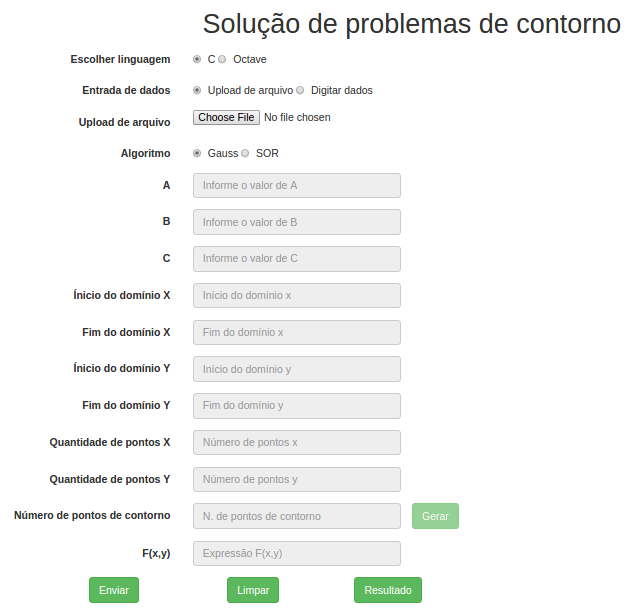
\includegraphics[width=\textwidth]{interface.png}
\centering
\caption{Interface \textit{web}}
\label{fig:interface}
\end{figure}

Também é possível executar o programa em modo texto, porém em módulos separados da linguagens. \textit{Pré-requisito}: ter o lua instalado. Para instalar o lua, pode-se executar \textit{make linux install} na pasta do lua anexada ao trabalho.

Em C, executa-se da seguinte forma:

./trab2 [Algoritmo] [Metodo de Entrada] [Arquivo?] [Omega?] [Tolerancia?]

Onde em \textbf{Algoritmo} insere-se \textit{gauss} ou \textit{sor}; em \textbf{Método de Entrada}, \textit{-t} para teclado ou \textit{-f} e o \textit{arquivo} a ser executado; e caso o algoritmo seja o SOR, insere-se os parâmetros de \textit{relaxação} e \textit{tolerância}.

Em Octave, deve-se executar o seguinte:

octave --silent --eval ``trab('[Algoritmo]',[Omega?])'' -qf

Onde o arquivo de entrada deve estar numa pasta um diretório acima e se chamar ``\textit{input.txt}''.

% ----------------------------------------------------------
% Experimentos Numéricos
% ----------------------------------------------------------
\section{Experimentos Numéricos}
Serão apresentados agora os testes realizados para a validação dos algoritmos desenvolvidos.

\subsection{\textit{Hardware} utilizado}
Os testes nesta seção foram executados em uma máquina com as seguintes configurações:

Linux Mint 17.2 Cinnamon 64-bit \\
\indent Intel Core i7-3770 CPU @ 3.40GHz x 4 \\
\indent 8GB de memória

\subsection{Testes}
A seguir serão caraterizados os dois testes realizados. Foram aplicados para as malhas $8 \times 8$, $16 \times 16$, $32 \times 32$, $64 \times 64$, $128 \times 128$ e $256 \times 256$ o teste 2 e apenas as duas primeiras malhas para o teste 1.

\subsubsection{\textit{test1}: Equação de Laplace}
Um caso simples de aplicação é a condução de calor em uma placa plana com condições de contorno constantes e iguais. Em condições ideias de condutividade a variação da temperatura $T(x,y)$ em uma placa retangular satisfaz a equação de Laplace, um caso particular da equação \eqref{eq:1}:

\begin{equation} \label{eq:2}
- \left(\frac{\partial^2 u}{\partial x^2} + \frac{\partial^2 u}{\partial y^2}\right) = 0
\text{ em } (x_0,x_{N+1}) \times (y_0,y_{M+1})
\end{equation}

Ou seja, neste caso temos que $ a = b = c = 0 $ e $ f(x,y) = 0 $.

Veja na figura \ref{fig:1} o gráfico do teste Laplace com uma malha $8\times8$ e valores de contorno iguais à 1.

\begin{figure}[h]
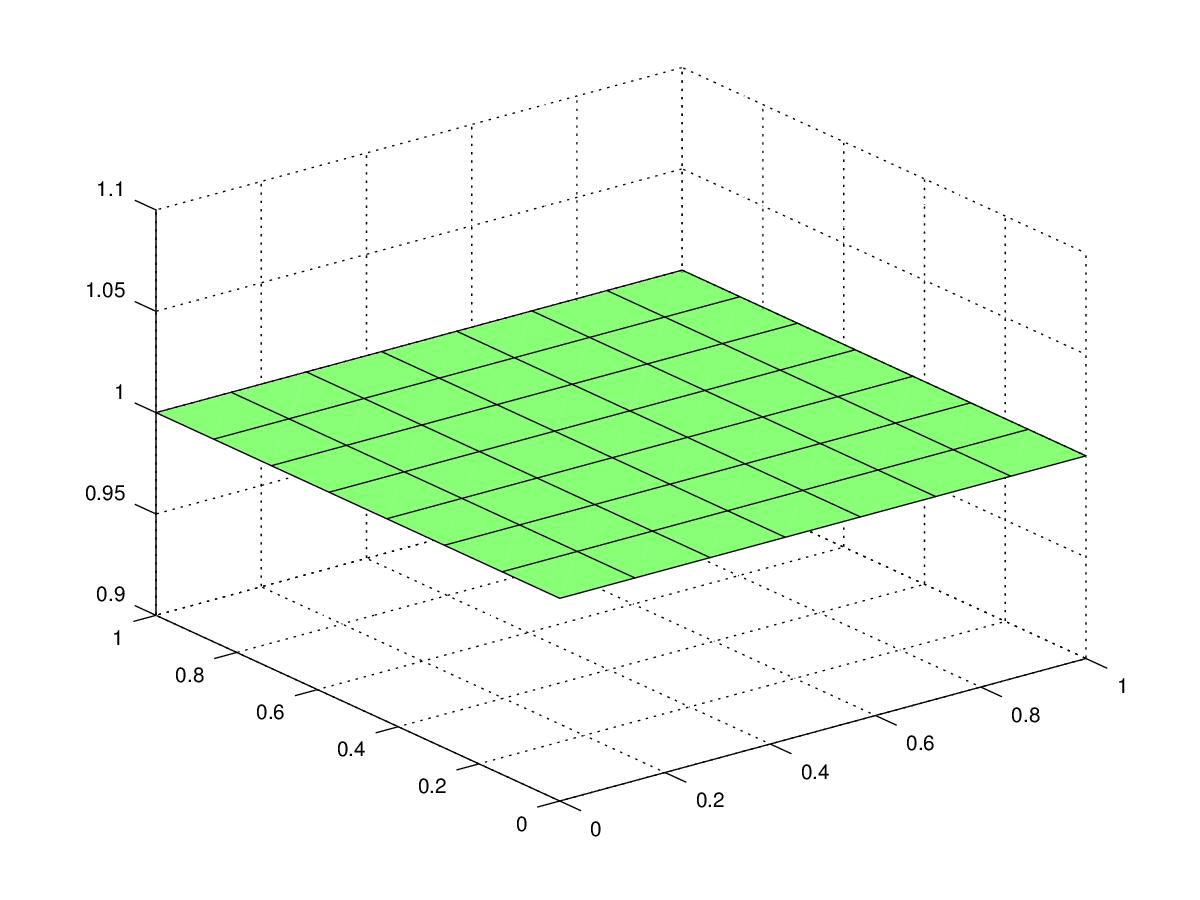
\includegraphics[width=\textwidth]{laplace-8x8.jpg}
\centering
\caption{Teste Laplace $8\times8$ e contorno igual a 1}
\label{fig:1}
\end{figure}

Como esperado, devido à equação de Laplace, todos os valores da malha resultaram em 1.

Em outro teste, também de malha $8\times8$, valoramos o contorno da malha com valores diferentes: 10 e 20. Veja o gráfico resultante na figura \ref{fig:1-2}.

\begin{figure}[h]
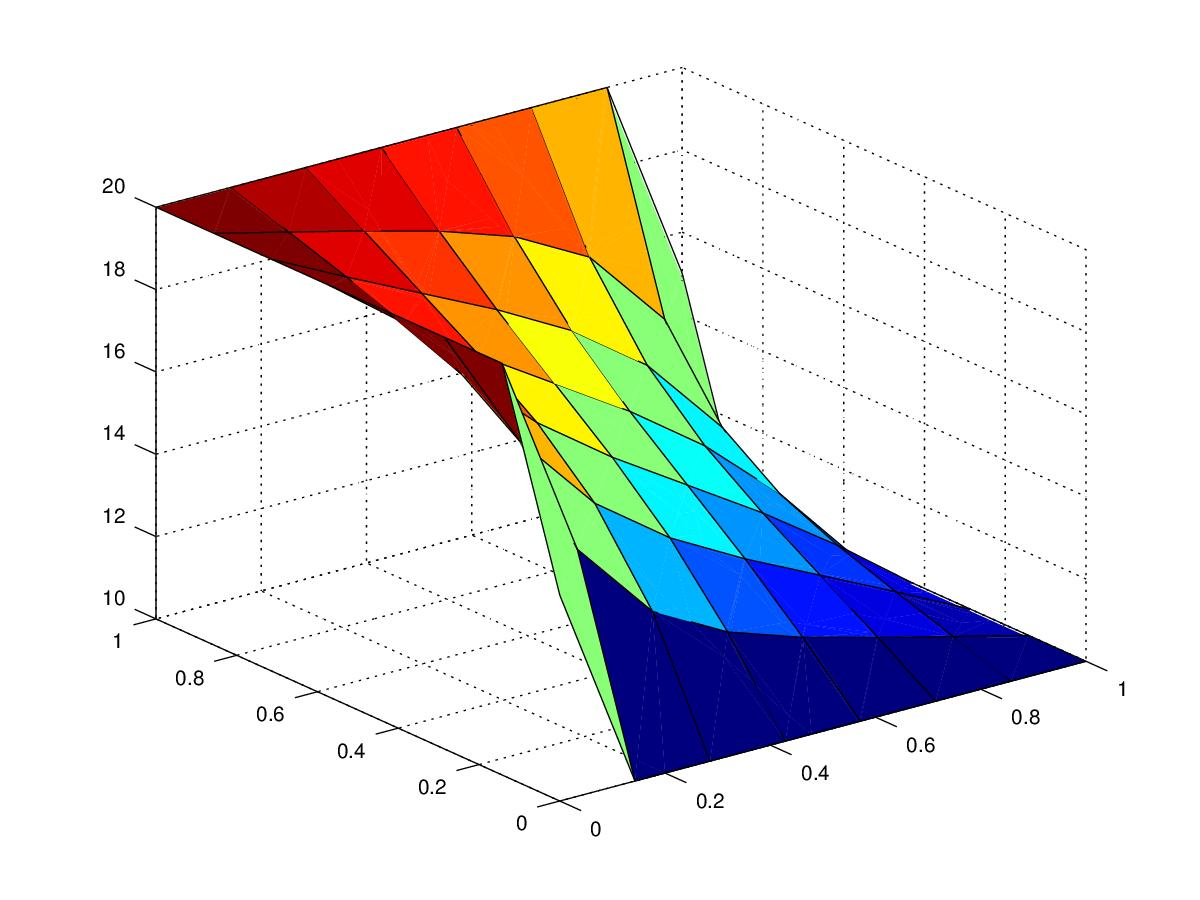
\includegraphics[width=\textwidth]{laplace-8x8-2.jpg}
\centering
\caption{Teste Laplace $8\times8$ e contorno 10 e 20}
\label{fig:1-2}
\end{figure}

\subsubsection{\textit{test2}}
Para este teste, temos as seguintes configurações: Considere a equação \eqref{eq:1} em $ \Omega = \left\{(x,y) : 0 \le x,y \le 1\right\} $ onde $a = 60$, $b = 80$, $c = -40$ e $f(x,y)$ é tal que $u(x,y) = xe^{xy}sen(\pi x)cos(\pi y)$.

Veja na figura \ref{fig:2} o gráfico deste teste com uma malha $8\times8$ e valores de contorno aplicados na função $u(x,y)$.

\begin{figure}[h]
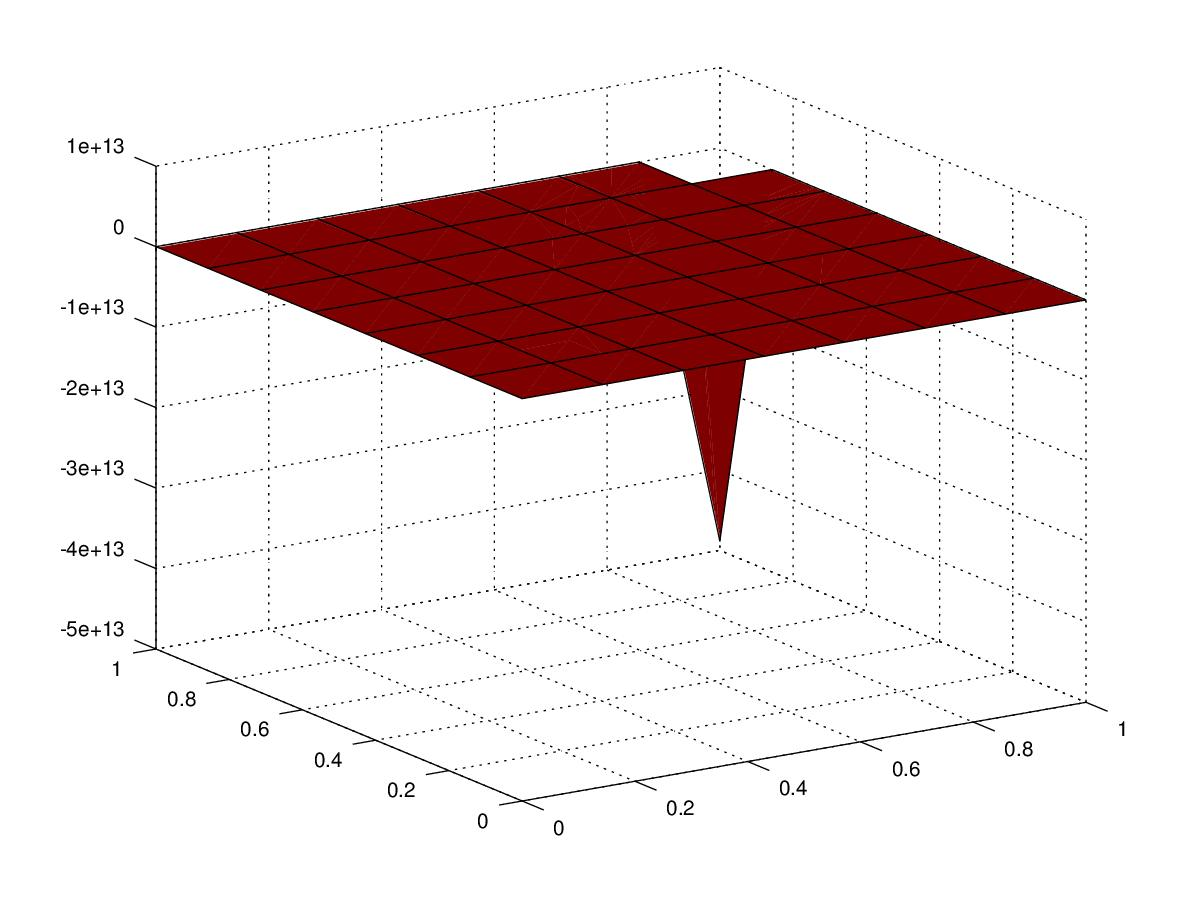
\includegraphics[width=\textwidth]{outros-8x8.jpg}
\centering
\caption{Teste 2 com malha $8\times8$}
\label{fig:2}
\end{figure}

\subsection{Comparações}
Veja as tabelas \ref{tab:cmp1} e \ref{tab:cmp2}, dos testes 1 e 2, respectivamente, de comparação entre os algoritmos e as linguagens em questão de eficiência.

\begin{table}[ht]
\centering
\begin{tabular}{cccc}
\hline 
\textbf{Malha} & \textbf{Linguagem} & \textbf{Algoritmo} & \textbf{Tempo de execução} \\
\hline
\multirow{4}{*}{\textit{$8 \times 8$}} & \multirow{2}{*}{C}  & Gauss & 0.002s  \\ 
& & SOR & 0.002s  \\
& \multirow{2}{*}{Octave} & Gauss & 1.158s  \\
& & SOR & $\infty$ \\
\hline
\multirow{4}{*}{\textit{$16 \times 16$}} & \multirow{2}{*}{C} & Gauss & 0.017s  \\ 
& & SOR & 0.006s  \\
& \multirow{2}{*}{Octave} & Gauss & 1m1.133s  \\
& & SOR & $\infty$ \\
\hline
\end{tabular}
\caption{Comparações do \textit{test1}}
\label{tab:cmp1}
\end{table}

\begin{table}[ht]
\centering
\begin{tabular}{cccc}
\hline 
\textbf{Malha} & \textbf{Linguagem} & \textbf{Algoritmo} & \textbf{Tempo de execução} \\
\hline
\multirow{4}{*}{\textit{$8 \times 8$}} & \multirow{2}{*}{C}  & Gauss & 0.002s  \\ 
& & SOR & 0.003s  \\
& \multirow{2}{*}{Octave} & Gauss & 1.151ss  \\
& & SOR & $\infty$ \\
\hline
\multirow{4}{*}{\textit{$16 \times 16$}} & \multirow{2}{*}{C} & Gauss & 0.022s  \\ 
& & SOR & 0.008s  \\
& \multirow{2}{*}{Octave} & Gauss & 1m0.799s  \\
& & SOR & $\infty$ \\
\hline
\multirow{4}{*}{\textit{$32 \times 32$}} & \multirow{2}{*}{C} & Gauss & 0.346s  \\ 
& & SOR & 0.034s  \\
& \multirow{2}{*}{Octave} & Gauss & $\infty$  \\
& & SOR & $\infty$ \\
\hline
\multirow{4}{*}{\textit{$64 \times 64$}} & \multirow{2}{*}{C} & Gauss & 19.602s  \\ 
& & SOR & 0.172s  \\
& \multirow{2}{*}{Octave} & Gauss & $\infty$  \\
& & SOR & $\infty$ \\
\hline
\multirow{4}{*}{\textit{$128 \times 128$}} & \multirow{2}{*}{C} & Gauss & $\infty$  \\ 
& & SOR & 1.603s  \\
& \multirow{2}{*}{Octave} & Gauss & $\infty$  \\
& & SOR & $\infty$ \\
\hline
\multirow{4}{*}{\textit{$256 \times 256$}} & \multirow{2}{*}{C} & Gauss & $\infty$  \\ 
& & SOR & $\infty$  \\
& \multirow{2}{*}{Octave} & Gauss & $\infty$  \\
& & SOR & $\infty$ \\
\hline
\end{tabular}
\caption{Comparações do \textit{test2}}
\label{tab:cmp2}
\end{table}

Através dos testes completados, vemos que a solução de problemas de valor de contorno bidimensionais é um processo muito custoso mesmo para casos aparentemente pequenos. Por exemplo, uma malha $16\times16$ gera uma matriz esparsa penta-diagonal de ordem \textit{256}, e uma malha $256\times256$ geraria uma matriz de ordem \textit{65536}. O que remete à importância do tratamento especial esparso.

É possível afirmar também que os algoritmos em C são significantemente mais rápidos devido à complexidade da linguagem se comparado ao Octave.

Infelizmente, não foi possível realizar muitos dos testes propostos por inviabilidade do sistema. Os casos de malha 32 para cima geravam entradas, ao aplicar na $u(x,y)$, inviáveis ao sistema, resultando assim em saídas corrompidas e nada aceitáveis. Porém ainda registramos os tempos de processamento destes casos. Os tempos marcados como $\infty$ significam que o processo foi longo demais para ser anotado.

% ----------------------------------------------------------
% Conclusão
% ----------------------------------------------------------
\section{Conclusão}
Podemos ver que encontrar o resultado de equações diferenciais não é uma tarefa tão trivial, porém algo muito utilizado e útil. Os sistemas penta-diagonais com os quais estamos trabalhando, podem ser muito complexos de serem gerados e resolvidos. Em nosso caso, consideramos a, b e c como constantes, o que facilitou a montagem da matriz penta-diagonal, no entanto, nem por isso se tornou um sistema simplório de se resolver. Também pode ser observado que quanto maior a discretização do domínio, terei mais precisão na malha, consequentemente, sabe-se o valor de mais pontos na malha. Pode ser visto, que resolver equações de Laplace são muito mais simples de serem resolvidas.

Para os problemas de contorno é essencial boas técnicas de arrendondamento, e boas formas de otimização para a resolução de sistemas esparsos, devido a malhas muito grandes gerarem sistemas enormes, no qual $N \times M$ é a ordem da matriz do sistema, e com isso podendo levar a divergência do sistema muito rápido no \textit{sor}, e várias horas de cálculos sem sucesso no \textit{gauss}. Também pode ser observado, que a linguagem Octave é muito mais simples, sendo assim aconselhável sua utilização para resolver vários problemas, mesmo possuindo execução mais lenta.

Por fim, através de nossos testes, podemos afirmar que a resolução de problemas de contorno de modo iterativo, pode alcançar resultados bons e mais rapidamente, porém da mesma forma, pode não alcançar resultados satisfatórios para outros caso, sendo assim de suma importância uma boa estratégia para a abordagem do problema de resolução de matrizes esparsas.

% ----------------------------------------------------------
% Referências bibliográficas
% ----------------------------------------------------------
\bibliography{trab2}{}
\bibliographystyle{ieeetr}
\addcontentsline{toc}{section}{Referências}

\end{document}
